\documentclass[tikz,border=8pt]{standalone}
% Requer xelatex e a fonte Poppins. Ajuste o Path abaixo (ou use \setmainfont{Poppins} se ela estiver instalada).
\usepackage{fontspec}
\setmainfont{Poppins}[Path=/usr/share/fonts/truetype/google-fonts/,Extension=.ttf,UprightFont=*-Regular,BoldFont=*-Bold,ItalicFont=*-Italic,BoldItalicFont=*-BoldItalic]
\usepackage{xcolor}
\definecolor{azulescuro}{HTML}{4A6F9C}
\definecolor{azulmedio}{HTML}{6F93BC}
\definecolor{azulclaro}{HTML}{E9EDF3}
\definecolor{azulsenac}{HTML}{1F4E9A}
\definecolor{laranja}{HTML}{F19E37}
\definecolor{laranjaescuro}{HTML}{D9731A}
\definecolor{laranjaclaro}{HTML}{FDEFD9}
\definecolor{cinzatitulo}{HTML}{333333}
\definecolor{cinzatexto}{HTML}{5C5C5C}
\usepackage{tikz}
\usetikzlibrary{positioning,arrows.meta,fit,backgrounds,calc}

\begin{document}
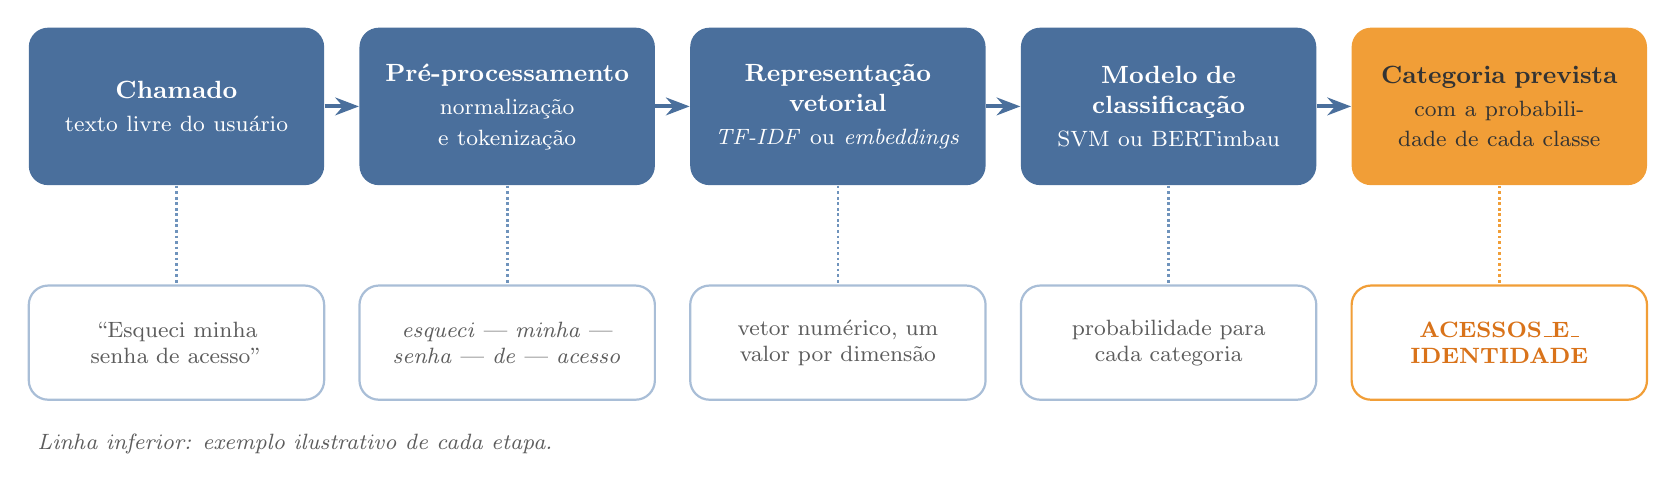
\begin{tikzpicture}[
    font=\small\color{cinzatexto},
    etapa/.style={fill=azulescuro, text=white, rounded corners=7pt, align=center, minimum height=2.0cm, text width=3.4cm, inner sep=5pt},
    final/.style={etapa, fill=laranja, text=cinzatitulo},
    ex/.style={draw=azulmedio!60, fill=white, thick, rounded corners=7pt, align=center, minimum height=1.45cm, text width=3.4cm, inner sep=5pt, font=\footnotesize\color{cinzatexto}},
    exf/.style={ex, draw=laranja},
    seta/.style={-{Stealth[length=3mm]}, line width=1.4pt, color=azulescuro},
    lig/.style={densely dotted, line width=1pt, color=azulmedio}
]
\def\dx{4.2}
\node[etapa] (a) at (0*\dx,0) {{\bfseries Chamado}\\[1pt]{\footnotesize texto livre do usuário}};
\node[etapa] (b) at (1*\dx,0) {{\bfseries Pré\mbox{-}processamento}\\[1pt]{\footnotesize normalização e tokenização}};
\node[etapa] (c) at (2*\dx,0) {{\bfseries Representação vetorial}\\[1pt]{\footnotesize \textit{TF-IDF} ou \mbox{\textit{embeddings}}}};
\node[etapa] (d) at (3*\dx,0) {{\bfseries Modelo de classificação}\\[1pt]{\footnotesize SVM ou BERTimbau}};
\node[final] (e) at (4*\dx,0) {{\bfseries Categoria prevista}\\[1pt]{\footnotesize com a probabilidade de cada classe}};
\foreach \i/\j in {a/b,b/c,c/d,d/e}{\draw[seta] (\i) -- (\j);}
\node[ex] (a2) at (0*\dx,-3.0) {“Esqueci minha senha de acesso”};
\node[ex] (b2) at (1*\dx,-3.0) {\textit{esqueci} | \textit{minha} | \textit{senha} | \textit{de} | \textit{acesso}};
\node[ex] (c2) at (2*\dx,-3.0) {vetor numérico, um valor por dimensão};
\node[ex] (d2) at (3*\dx,-3.0) {probabilidade para cada categoria};
\node[exf] (e2) at (4*\dx,-3.0) {\bfseries\footnotesize\color{laranjaescuro} ACESSOS\_E\_\allowbreak IDENTIDADE};
\foreach \i in {a,b,c,d}{\draw[lig] (\i.south) -- (\i2.north);}
\draw[lig, color=laranja] (e.south) -- (e2.north);
\node[font=\footnotesize\itshape\color{cinzatexto}, anchor=west] at ($(a2.south west)+(0,-0.55)$) {Linha inferior: exemplo ilustrativo de cada etapa.};
\end{tikzpicture}
\end{document}
